\section{Химическая и биологическая эволюция. Наследственность, изменчивость и естественный отбор. Основные таксономические группы живых систем. Строение клетки про- и эукариот (сходства и различия). Единство молекулярных механизмов живых систем (примеры). Организация генома живых существ: хромосомы, ДНК пластид и митохондрий, плазмиды.}

\subsection{Химическая эволюция и биологическая эволюция}

\textbf{Химическая эволюция} --- этап, предшествовавший появлению жизни, в ходе которого органические, пребиотические вещества возникали из неорганических молекул под влиянием внешних энергетических и селекционных факторов и в силу развертывания процессов самоорганизации, свойственных всем относительно сложным системам, которыми, бесспорно, являются все углеродосодержащие молекулы.

\medspace

Пребиотический синтез сложных соединений молекул может делиться на три этапа:

\begin{enumerate}
	\item Возникновение простых органических соединений (спиртов, кислот и т.п.) из неорганических;
	
	\item Синтез более сложных органических соединений — <<биомолекул>> — представителей наиболее распространённых классов метаболитов (продукты метаболизма), в том числе и мономеров --- структурных единиц биополимеров (моносахаридов, аминокислот, жирных кислот, нуклеотидов) из простых органических соединений;
	
	\item Возникновение сложных биополимеров (полисахариды, белки, нуклеиновые кислоты) из основных структурных единиц --- мономеров.
\end{enumerate}

\textbf{Биологическая эволюция} --- любое генетическое изменение в популяции, которое происходило в течение нескольких поколений. Изменения должны происходить на генетическом уровне вида и передаваться от одного поколения к другому.

\subsection{Наследственность, изменчивость и естественный отбор}

\textbf{Наследственность} --- способность организмов передавать свои признаки и особенности развития потомству. Благодаря ей живые существа сохраняют в своих потомках характерные черты вида. Наследственность обеспечивается передачей генетической информации. Например, у эукариот материальными единицами наследственности являются гены, локализованные в хромосомах ядра и ДНК органелл.

\textbf{Изменчивость} --- разнообразие признаков среди представителей данного вида, а также свойство потомков приобретать отличия от родительских форм.

Изменчивость бывает нескольких типов. Выделим парочку:

\begin{itemize}
	\item Наследственная (обусловлена возникновением разных типов мутаций и их комбинаций, которые передаются по наследству и впоследствии проявляются у потомства) и ненаследственная (способность организмов с одинаковым генотипом развиваться по-разному в разных условиях окружающей среды);
	
	\item Индивидуальная (различие между отдельными особями) и групповую (различия между группами особей, например, различными популяциями вида, является производной от индивидуальной).
\end{itemize}

\textbf{Естественный отбор} --- основной фактор эволюции, в результате действия которого в популяции увеличивается число особей, обладающих более высокой приспособленностью к условиям среды (наиболее благоприятными признаками), в то время как количество особей с неблагоприятными признаками уменьшается.

\subsection{Основные таксономические группы живых систем}

Таксономическая группа фактически это уровень в биологической систематике, т.е. в дисциплине, которая разрабатывает принципы классификации живых организмов. Таксоны идут по иерархии, представим ее от более глобальных таксонов к менее глобальным (только основные, иначе можно с ума сойти; в скобках --- название на латыни):

\begin{itemize}
	\item Царство (regnum);
	
	\item Тип (phylum) --- у растений вместо него Отдел (divisio);
	
	\item Класс (classis);
	
	\item Отряд (ordo) --- у растений вместо него Порядок (тоже ordo);
	
	\item Семейство (familia);
	
	\item Род (genus);
	
	\item Вид (species) --- группа организмов с общими морфофизиологическими, биохимическими и поведенческими признаками, способная к взаимному скрещиванию, которое даёт в ряду поколений плодовитое потомство, закономерно распространённая в пределах определённого ареала и сходно изменяющаяся под влиянием факторов внешней среды.
\end{itemize}

\subsection{Строение клетки про- и эукариот (сходства и различия)}

\begin{itemize}
	\item Размер клеток у прокариот сильно (в 1000 - 10000 раз) меньше, чем у эукариот;
	
	\item Прокариоты в основном одноклеточные, в то время как эукариоты все же в основном многоклеточные;
	
	\item Эукариоты сильно моложе (почти на 2 млрд лет) чем прокариоты (первые произошли от вторых);
	
	\item У прокариотов клетки в основном просто делятся пополам, в то время как у эукариотов возможны митозы, мейоз или их комбинация, при этом образуется т.н. веретено деления (т.е. динамическая структура, которая образуется в митозе и мейозе для обеспечения отделения хромосом и деления клетки);
	
	\item У прокариотов кольцевая ДНК просто плавает в цитоплазме, она не связана с белками или РНК, а хромосом нет. У эукариотов же ДНК линейная и локализована в ядре, имеются хромосомы, а днк связана с РНК и белком;
	
	\item У прокариот мелкие (70S) рибосомы, эндоплазматического ретикулума (это внутриклеточный органоид эукариотической клетки, который представляет из себя разветвленную систему из окруженных мембраной уплощенных полостей пузырьков и канальцев) нет (различия и по многим другим деталям белкового синтеза, включая чувствительность к антибиотикам; синтез белков у прокариот, например, подавляется антибиотиком стрептомицином). У эукариот же крупные (80S) рибосомы, которые могут быть прикреплены к эндоплазматическому ретикулуму;
	
	\item Органелл у прокариот мало, ни одна из них не имеет оболочки (двойной мембраны). Внутренних мембран почти нет, редко, когда они есть, их ассоциируют с процессами дыхания и фотосинтеза. У эукариот наоборот (органеллы это например ядро, митохондрии, хлоропласты);
	
	\item Клеточные стенки у прокариот жесткие, содержат полисахариды и аминокислоты, основной опорный материал --- муреин (компонент, выполняющий функцию осмотической защиты клетки). У эукариот бывает по-разному: у зеленых растений и грибов стенки жесткие, содержат полисахариды. У растений они в основном из целлюлозы, у грибов из хитина. У животных клеточной стенки нет;
	
	\item У прокариот жгутики простые, нет микротрубочек (белковые внутриклеточные структуры, входящие в состав цитоскилета, которые представляют собой полые цилиндры диаметром 25 нм. Длина может варьироваться), расположены внеклеточно (не окружены плазматической мембраной). У эукариот же жгутики они сложные, окружены плазматической мембраной. Диаметр их раз в 10 больше;
	
	\item Дыхание у прокариот происходит в мезосомах, у цианобактерий --- на цитоплазматических мембранах. У эукариот же аэробное дыхание, которое происходит в митохондриях;
	
	\item У прокариот не бывает хлоропластов, а фотосинтез (если есть) происходит на мембранах, у которых нет специфической упаковки. У эукариот же появляются хлоропласты (если они делают фотосинтез), состоящие из уложенных в особую структуру мембран;
	
	\item Некоторые прокариоты могут фиксировать азот. Эукариоты так не умеют.
	
\end{itemize}


\subsection{Единство молекулярных механизмов живых систем (примеры)}

Хз. Примеры например:

\begin{itemize}
	\item Единый генетический код;
	
	\item Большинство состоят из клеток (кроме вирусов), которые схожи по внутреннему строению.
\end{itemize}

\subsection{Организация генома живых существ: хромосомы, ДНК пластид и митохондрий, плазмиды}

\subsubsection{Хромосомы}

Вытянутые, структурированные совокупности генов, которые несут информацию о наследственности и образованы и конденсированного хроматина (масса генетического материала, состоящая из ДНК и белков, которые конденсируются с образованием хромосом во время деления эукариотических клеток. Хроматин содержится в ядрах клеток). Наборы хромосом соединяются вместе (один от отца, один от матери) и известны как гомологические хромосомы (пары хромосом, одинаковые по длине, положению генов и местоположению центромеров).

\begin{figure}[H]
	\centering
	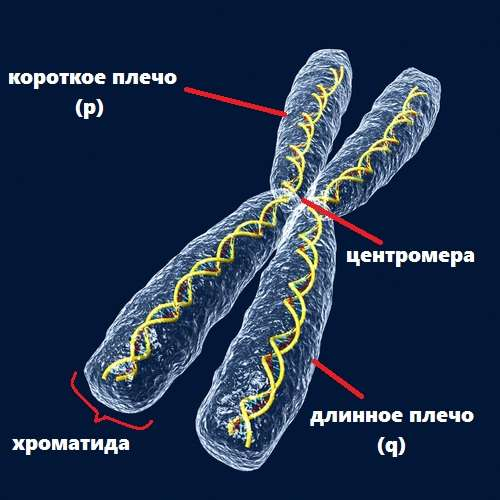
\includegraphics[width=0.7\linewidth]{1_chromosome}
	\caption{Строение хромосомы}
\end{figure}

\subsubsection{ДНК пластид и митохондрий}

И митохондрии, и пластиды --- двухмембранные органоиды эукариотических клеток. Митохондрии встречаются во всех клетках животных и растений, пластиды же характерны для клеток растений, осуществляющих фотосинтетические процессы. Эти органоиды имеют сходный план строения и некоторые общие свойства. Однако по основным метаболическим процессам они существенно отличаются друг от друга.

\begin{itemize}
	\item \textbf{Митохондрии} --- округлые, овальные или палочковидные двухмембранные органоиды диаметром около 0.21 мкм и длиной до 710 мкм. Основная --- функция синтез АТФ.
	
	\item \textbf{Пластиды} --- двухмембранные органоиды, характерные для фотосинтезирующих эукариотных организмов. Различают три основных типа пластид: хлоропласты, хромопласты и лейкопласты. Совокупность пластид в клетке называют пластидомом. Каждый из этих типов при определенных условиях может переходить один в другой. Как и митохондрии, пластиды содержат собственные молекулы ДНК. Поэтому они также способны размножаться независимо от деления клетки.
	
	Пластиды бывают разные:
	
	\begin{itemize}
		\item \textbf{Хлоропласты} --- пластиды, в которых осуществляется фотосинтез.
		
		\item \textbf{Хромопласты} --- окрашенные пластиды. Цвет их обусловлен наличием следующих пигментов: каротина (оранжевожелтый), ликопина (красный) и ксантофилла (желтый). Хромопластов особенно много в клетках лепестков цветков и оболочек плодов.
		
		\item \textbf{Лейкопласты} --- бесцветные пластиды округлой, яйцевидной, веретенообразной формы. Находятся в подземных частях растений, семенах, эпидермисе, сердцевине стебля. Основная функция лейкопластов --- это аккумуляция питательных веществ.
	\end{itemize}
\end{itemize}

Теперь немного про их ДНК. Их характерные черты:

\begin{itemize}
	\item Митохондрии и пластиды имеют собственную специфическую систему синтеза белков (ДНК, РНК, рибосомы). Специфичность этой системы заключается в автономности и резком отличии от таковой в клетке;
	
	\item ДНК митохондрий и пластид представляет собой небольшую циклическую или линейную молекулу, которая отличается от ДНК ядра и по своим характеристикам приближается к ДНК прокариотических клеток. Синтез ДНК митохондрий и пластид не зависит от синтеза ядерной ДНК;
	
	\item В митохондриях и хлоропластах имеются иРНК (информационная), тРНК (транспортная), рРНК (рибосомная). Рибосомы и рРНК этих органоидов резко отличаются от таковых в цитоплазме. В частности рибосомы митохондрий и хлоропластов, в отличие от цитоплазматических рибосом, чувствительны к антибиотику хлорамфениколу, подавляющему синтез белка у прокариотических клеток.
\end{itemize}

\subsubsection{Плазмиды}

Это небольшие молекулы ДНК, физически обособленные от хромосом и способные к автономной репликации. Главным образом плазмиды встречаются у бактерий, а также у некоторых архей и эукариот (грибов и высших растений). Чаще всего плазмиды представляют собой двухцепочечные кольцевые молекулы. Несмотря на способность к размножению, плазмиды, как и вирусы, не рассматриваются в качестве живых организмов. Плазмиды в основном кодируют функции, придающие бактерии преимущество в случае попадания в неблагоприятные условия (например, устойчивость к антибиотикам или, наоборот, синтез антибиотических веществ).

Размеры плазмид варьируют от менее чем 1 тысячи до 400—600 тысяч пар оснований (п. о.). Некоторые плазмиды содержатся в клетке в количестве однойдвух копий, другие — в количестве нескольких десятков. Плазмиды разных классов могут сосуществовать в клетке.

\begin{figure}[H]
	\centering
	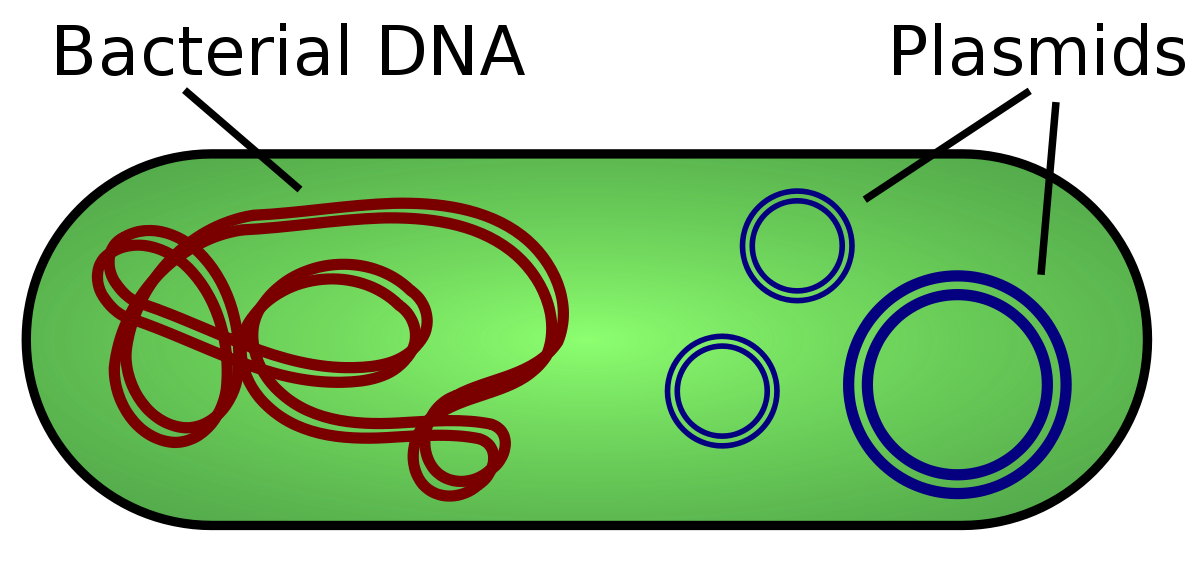
\includegraphics[width=0.7\linewidth]{1_plazmids}
	\caption{Плазмиды и хромосомная ДНК в бактериальной клетке}
\end{figure}































